\documentclass{article}
\usepackage{graphicx}
\usepackage{mathtools}
\usepackage{xfrac}
\usepackage{amsmath, amssymb}
\usepackage{listings}
\usepackage{float}
\usepackage{wrapfig}
\usepackage{tikz}
\usepackage{fullpage}
\usepackage{hyperref}
\usepackage{mathalpha}
\usepackage{tikz}
\usepackage{cite}
\usepackage{amsthm}


\title{Molecular Spectroscopy}
\author{David Lawton, TCD\\Student No. 22337087\\ Lab Partner: Sami Lopez-Steffenson}
\date{4th Oct. 2024.}

\begin{document}

\maketitle

\tableofcontents

\newpage

\section{Abstract}

\section{Introduction}
\begin{wrapfigure}{r}{0.5\textwidth}
    \centering
    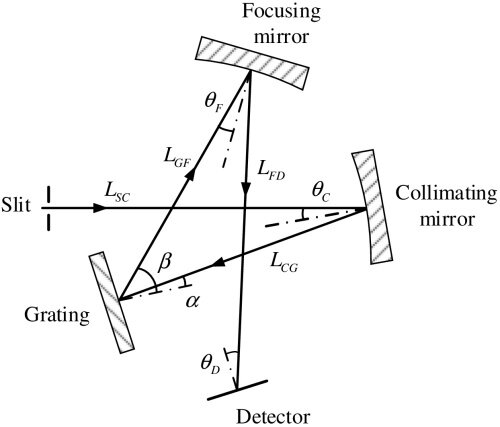
\includegraphics[width=0.5\textwidth]
    {/home/dj-lawton/Documents/Junior Sophister/JS Labs/Molecular Spectroscopy/Images/Crossed-Czerny-TurnerType.jpg}
    \caption{\label{fig:crossedCzernyTurner}A diagram of a crossed Czerny-Turner Type Spectrometer's optical bench.\cite{article}}
\end{wrapfigure}
This report details the experimental procedure and results of the Molecular Spectroscopy lab. The aim of the experiment was to learn about the principles of optical emission and absorption spectroscopy, and the molecules being analysed. The experiment was conducted using two computerised diffraction grating spectrometers, of crossed Czerny-Turner type, with a $50\mu m$ diameter optical fibre input. The output is displayed digitally using the software provided.

\subsection{Theory \& Background}
Unlike the lines of atomic emission spectra, which are due to transitions between electronic energy level, molecular emission spectra are due to transitions between vibrational and rotational energy levels, as well as electronic. In this experiment we are concerned with only the \textbf{vibronic} transitions, which are transitions between vibrational and electronic energy levels, due to insufficiently high resolution to view rotational energy levels.\\
\indent While the electronic levels are described similarly to that of an atom, we must use a different model for the vibrational levels.\\
\subsubsection{Molecular Vibrations}
\indent It would seem natural to first consider the harmonic oscillator model for molecular vibrations, which is a decent approximation for small vibrations. The potential dictating this being
\begin{equation}
    V(x) = \frac{1}{2}kx^2
\end{equation}
Which yields the energy levels:
\begin{equation}
    E_{\nu} = \left(\nu + \frac{1}{2}\right)\hbar\omega
\end{equation}
Where $\nu$ is the vibrational quantum number, and $\omega = \sqrt{\frac{k}{\mu}}$ is the fundamental frequency of the oscillation. Here, $k$ is the spring constant of the vibration, $\mu$, the reduced mass, which is used when describing the sytem to reduce it from a two body problem to a one body problem.\\
\indent Since rotational and vibrational energy levels are usually expressed in terms of wavenumber, we can convert the above to wavenumber by dividing by $hc$, where $h$ is Planck's constant and $c$ is the speed of light. This gives us the formula:
\begin{equation}
    G(\nu)= \frac{E_{\nu}}{hc} = \left(\nu + \frac{1}{2}\right)\frac{\omega}{2\pi c}
\end{equation}
Now consider the $\frac{\omega}{2\pi c}$ term. \begin{align}
    \frac{\omega}{2\pi c}=& \frac{2\pi f}{2\pi c}\\ =& \frac{f}{c}\\ =& \frac{1}{\lambda} = \tilde{\nu}
\end{align}
where $\tilde{\nu}$ is the wavenumber, expressed in $m^{-1}$.\\
\indent We can now write the energy levels in wavenumbers as:
\begin{equation}
    G(\nu) = \left(\nu + \frac{1}{2}\right)\tilde{\nu}
    \label{eq: harmonicOscillator}
\end{equation}

\begin{wrapfigure}{r}{0.5\textwidth}
    \centering
    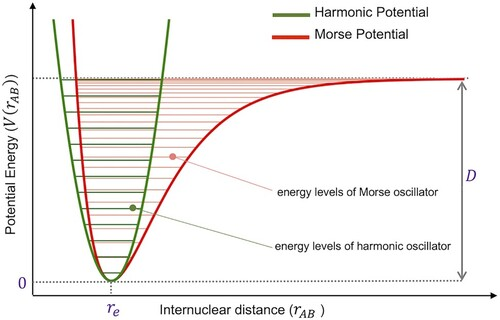
\includegraphics[width=0.5\textwidth]
    {/home/dj-lawton/Documents/Junior Sophister/JS Labs/Molecular Spectroscopy/Images/MorsePotential.jpg}
    \caption{\label{fig:morsePotential}A diagram of the Morse Potential.\cite{doi:10.1080/00268976.2024.2360542}}
\end{wrapfigure}

Unfortunately, the harmonic oscillator model is not a good approximation for larger vibrations. This is because the potential does not account for the fact that there is a finite energy $D_e$ which is the depth of the well. This is accounted for by the Morse potential\cite{doi:10.1080/00268976.2024.2360542}, which is given by:
\begin{equation}
    V(r) = D_e\left(1-e^{-\beta(r-r_e)}\right)^2
\end{equation}
where $r$ is the internuclear distance, $r_e$ is the equilibrium internuclear distance and $\beta$ is a constant defined by $\beta = \sqrt{\frac{k}{2D_e}}$. We can then write $\tilde{\nu}$ in terms of $\beta$ and $D_e$ as:
\begin{equation}
    \tilde{\nu} = \frac{\beta}{c}\sqrt{\frac{D_E}{2\pi^2 \mu}}
\end{equation}
Just as before, we solve the Schrodinger equation for the Morse potential\cite{1988JChPh..88.4535D} to find the energy levels, and convert to wavenumber.
\begin{equation}
    G^{\prime}(\nu) = \left(\nu + \frac{1}{2}\right)\tilde{\nu} - \left(\nu + \frac{1}{2}\right)^2\tilde{\nu}x_e 
\end{equation}
where $x_e$ is the anharmonicity constant.\\
\begin{equation}
    x_e = \frac{\tilde{\nu}}{4D_e}
\end{equation}
\indent The Morse Potential also allows transitions of $\delta\nu = \pm p$ to occur, where $p$ is an integer. These `overtones' are not allowed in the harmonic oscillator model\cite{21316}, and they occur because of the unequal spacing of energy levels in the anharmonic model.\\
\subsubsection{Molecular Bonding}
When molecules form, the atomic orbitals of the atoms involved combine to form molecular orbitals. These can be constructive or destructive, and the resulting molecular orbitals can be bonding or anti-bonding, respectively. The main difference between these is the fact that in anti-bonding orbitals, the electrons are less likely to be found in the region between the nuclei (exactly no likelihood at the nodal plane), and so the bond is weaker, as the electrons are more likely to be on opposite sides of the atoms, exerting a `pulling' effect. This is not the case for bonding orbitals.\\
The bonding wavefunction is given by:
\begin{equation}
    \psi_b = \frac{1}{\sqrt{2}}(\psi_1 + \psi_2)
\end{equation}
and the anti-bonding wavefunction is given by:
\begin{equation}
    \psi_{ab} = \frac{1}{\sqrt{2}}(\psi_1 - \psi_2)
\end{equation}
where $\psi_1$ and $\psi_2$ are the atomic orbitals of the atoms involved (Identical for homonuclear diatomic molecules).\\
\begin{wrapfigure}{r}{0.5\textwidth}
    \centering
    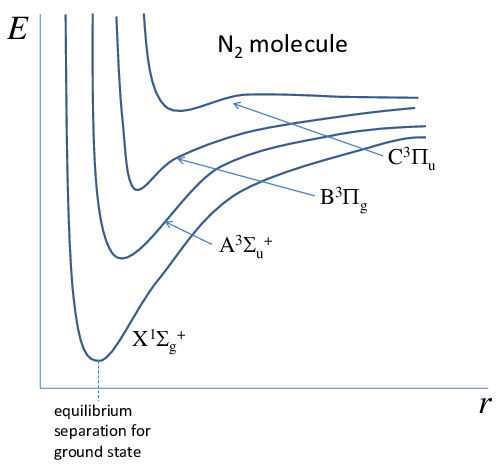
\includegraphics[width=0.5\textwidth]
    {/home/dj-lawton/Documents/Junior Sophister/JS Labs/Molecular Spectroscopy/Images/Nitrogen_Energies.png}
    \caption{\label{fig:N2MOs}The molecular orbitals of an $N_2$ molecule. We are mainly concerned with $C^3\Pi_u$ and $B^3\Pi_g$ in this experiment.\cite{unknown}}
\end{wrapfigure}
\indent One section of this experiment concerns the emission spectrum of an $N_2$ molecule. The $N_2$ molecule has a triple bond, and so the molecular orbitals are formed from the $2s$ and $2p$ orbitals of the nitrogen atoms. As can be seen in figure \ref{fig:N2MOs}, the $C^3\Pi_u$ and $B^3\Pi_g$ orbitals are the 3rd and 2nd energy orbitals, respectively (from 0th), where $\Pi$ refers to the type of orbitals superimposed, and the u, g refer to ungerade and gerade. Molecular orbitals with the g subscript are bonding orbitals (symmetric), while those with the u subscript are anti-bonding orbitals (antisymmetric). The $C^3\Pi_u$ orbital corresponds to the anti-bonding orbitals of the $2p$ orbitals, while the $B^3\Pi_g$ corresponds to the bonding orbitals. It is clear then that the $C^3\Pi_u$ orbitals are higher in energy than the $B^3\Pi_g$ orbitals, due to their asymmetry. It also clearly portrays the instability of the anti-bonding orbitals, as the $C^3\Pi_u$ curve has a markedly shallower potential well than $B^3\Pi_g$.\\
\subsubsection{Vibronic Transitions, Franck-Condon Factors}
We know already that $\Delta n = \pm 1$ for electronic transitions, where n is the electronic quantum number. For vibrational transitions,  this is not the case. The Franck-Condon principle states that an electronic transition is most likely to occur without changes in the positions of the nuclei in the molecular entity and its environment (vibrational, external motion)(Figure \ref{fig:FranckCondon}). The quantum mechanical formulation of this principle is that the intensity of a vibronic transition is proportional to the square of the overlap integral between the vibrational wavefunctions of the two states that are involved in the transition. 
\begin{equation}
    P_{mn} = |\langle \psi_{xm}|\boldsymbol{\mu}|\psi_{yn}\rangle|^2 \propto \left|\int \psi_{xm}^{\ast}(r)\psi_{yn}(r)dr\right|^2
\end{equation}
Where $P_{mn}$, the Franck-Condon factor, is the probability of a transition from the mth vibrational state of the initial electronic state to the nth vibrational state of the adjacent final electronic state, $\psi_{xm}$ is the wavefunction of the mth vibrational level in the xth electronic level, $\psi_{yn}$ is the wavefunction of the nth vibrational level in the yth electronic level, and $\boldsymbol{\mu}$ is the transition dipole moment operator.\\
\begin{wrapfigure}{r}{0.4\textwidth}
    \centering
    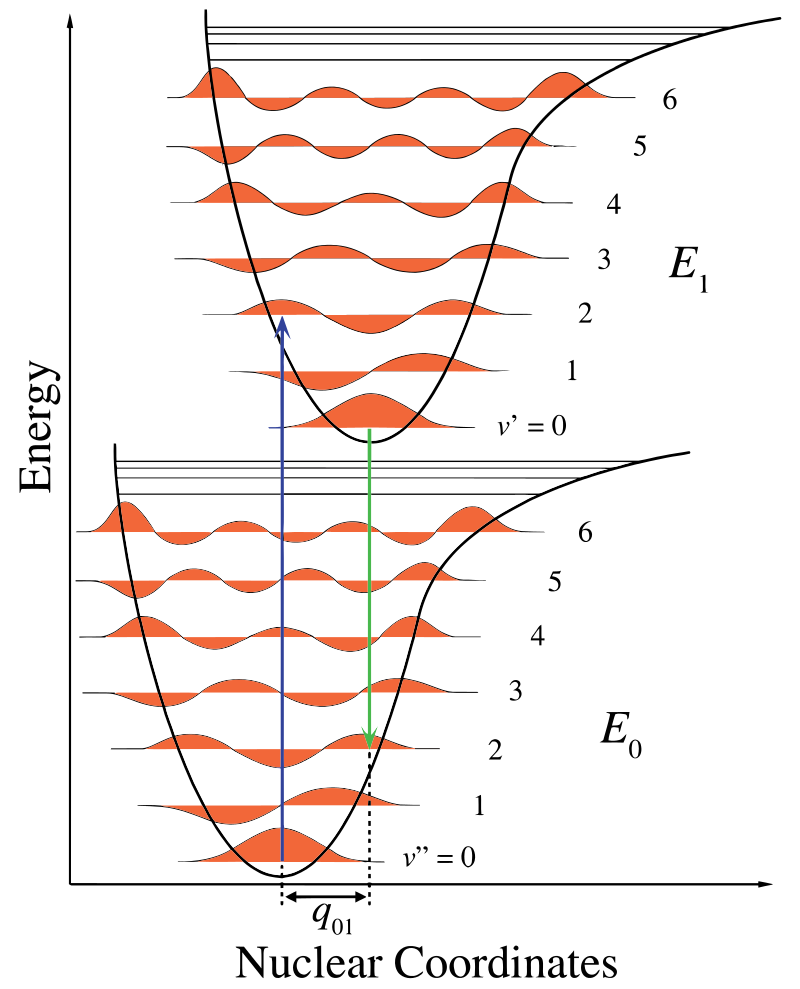
\includegraphics[width=0.35\textwidth]
    {/home/dj-lawton/Documents/Junior Sophister/JS Labs/Molecular Spectroscopy/Images/Franck_Condon.png}
    \caption{\label{fig:FranckCondon}A diagram illustrating the Franck-Condon Principle. Since the transitions are assumed to be vertical, vibrational levels with minimal change in $r$ are more likely to be involved in the transition.\cite{2023Franck}}
\end{wrapfigure}
The assumption we make that the transitions are vertical is a good one, as the timescale of the electronic transition is at a maximum, a few femtoseconds, while the timescale of the nuclear motion is at a minimum, 10s to hundreds of femtoseconds, while molecular motion is in the timescale of nanoseconds or larger. This means that the nuclei are essentially stationary during the electronic transition.\\
\indent A similar way to think about this is that electronic, atomic, and molecular frequencies of motion are to Gamma rays, X-rays, and visible light, respectively.\\
\indent It is also important to describe our notation for each transition. For the $N_2$ molecule, we are working with transitions between the $B^3\Pi_g$ and $C^3\Pi_u$ orbitals. We denote each transition as $i - j$, where $i$ is the initial vibrational level in the $C^3\Pi_u$ orbital, and $j$ is the final vibrational level in the $B^3\Pi_g$ orbital.\\

\subsection{Energy of Vibronic Transitions}
To predict the wavenumber of emitted spectral lines in vibronic transition, we must consider both the difference of energy between the two electronic states, and the difference in vibrational energy between the two states. By recognising, $\frac{\Delta E_{el}}{hc} = \tilde{\nu}_{el}$, where $\tilde{\nu}_{el}$ is the wavenumber of the emission due solely to the change in energy level, and subbing Eq. \ref{eq: harmonicOscillator}, we can write the energy of a vibronic transition as:
\begin{align}
    \tilde{\nu}_{\nu^{\prime}\nu^{''}} =& \frac{\Delta E_{el}}{hc}+\left(\frac{E_{\nu^{\prime}}}{hc}-\frac{E_{\nu^{''}}}{hc}\right)\\
    =& \tilde{\nu}_{el} + \tilde{\nu}_C\left[\left(\nu^{\prime}+\frac{1}{2}\right)-x_C\left(\nu^{\prime}+\frac{1}{2}\right)^2\right]-\tilde{\nu}_B\left[\left(\nu^{''}+\frac{1}{2}\right)-x_B\left(\nu^{''}+\frac{1}{2}\right)^2\right]
\end{align}
where the subscript C refers to the initial electronic state, $E_3$, and the subscript B refers to the final electronic state, $E_2$.\\
\indent We can then rearrange the equation to remove constant $\tilde{\nu}_{el}$, and write the equation in terms of the wavenumber of the $0-0$ transition:
\begin{equation}
    \tilde{\nu}_{\nu^{\prime}\nu^{''}} = \tilde{\nu}_{00} + \tilde{\nu}_C\nu^{\prime} - \tilde{\nu}_B\nu^{''} - \tilde{\nu}_Cx_C(\nu^{\prime}+1)\nu^{\prime} + \tilde{\nu}_Bx_B(\nu^{''}+1)\nu^{''}
\end{equation}
\indent We then, after measuring sufficiently many wavenumbers of peaks, are left with a solvable system of equations, with 4 unknowns, $\tilde{\nu}_C$, $\tilde{\nu}_B$, $x_C$, and $x_B$.
\begin{align}
    \begin{pmatrix}
        1 & 2\\
        2 & 6
    \end{pmatrix}
    \cdot
    \begin{pmatrix}
        \tilde{\nu}_B\\
        -\tilde{\nu}_Bx_B
    \end{pmatrix}
    =&
    \begin{pmatrix}
        1&\sfrac{1}{\tilde{\nu}_{02}}\\
        1&\sfrac{1}{\tilde{\nu}_{01}}
    \end{pmatrix}
    \cdot
    \begin{pmatrix}
        \tilde{\nu}_{00}\\
        -\tilde{\nu}_{01}\tilde{\nu}_{02}
    \end{pmatrix}\\
    \begin{pmatrix}
        2 & 1\\
        6 & 2
    \end{pmatrix}
    \cdot
    \begin{pmatrix}
        \tilde{\nu}_Cx_C\\
        -\tilde{\nu}_C\\
    \end{pmatrix}
    =&
    \begin{pmatrix}
        1&\sfrac{1}{\tilde{\nu}_{20}}\\
        1&\sfrac{1}{\tilde{\nu}_{10}}
    \end{pmatrix}
    \cdot
    \begin{pmatrix}
        \tilde{\nu}_{00}\\
        -\tilde{\nu}_{10}\tilde{\nu}_{20}
    \end{pmatrix}
\end{align}
This allows us to calculate one (or more) values of $\tilde{\nu}_C$, $\tilde{\nu}_B$, $x_B$, and $x_C$.  It is easier for us to calculate the values of $\tilde{\nu}_Cx_C$ and $\tilde{\nu}_Bx_B$ instead of $x_C$ and $x_B$ separately, as we can then calculate the dissociation energy of the molecule, $D_0$, simply, using the formula:
\begin{equation}
    \frac{D_0}{\hbar} = \frac{\tilde{\nu}^2}{4\tilde{\nu}x_B}
\end{equation}

\section{Methodology}
The general steps we took to setup for the procedure were first to ensure the spectrometer was connected to the computer, before turning on the computer and opening the software. We then carefully put the fibre optic cable corresponding to the spectrometer of lower threshold  into the higher clamp, used for observation.

\subsection{Calibration}
\label{sec:calibration}
The first section section of the procedure was the calibration of the spectrometers, which involved placing the calibration lamp (Mercury) directly facing the optical fibre (and wall).\\
\indent We varied the parameters of the sample, which were the integration time, the scans to average, the bin width, and correction for dark current, and noted the affects of varying each. We then tried to optimise our parameters for a low error, low noise sample. This involved keeping our integration time so that the maximum lied under the saturation point, since increasing the sample size reduces the effect of the noise, relative to the size of the sample. We also tried to do this while keeping a large number of scans to average, keeping bin widths small, and keeping electrical dark correction on.\\
\indent It followed only to capture the emission spectrum of mercury using the Flame-T spectrometer (lower threshold, $300-510nm$), swapped the optical fibres, and then captured the emission spectrum using the Flame-S spectrometer (higher threshold, $350-850nm$).\\
\indent We then use these spectrums to calibrate the spectrometers, by finding the peaks of the mercury spectrums using the code specified, and comparing them to the literature values. The optical resolution, resolving power of the spectrometers are found, and compared to expected values.\\
\indent 
\subsection{Emission Spectrum of $N_2$}
The second part of the experiment was to capture the emission spectrum of $N_2$ using the Flame-T spectrometer. This involved the use of an $N_2$ lamp, which was placed facing the wall, with the fibre optic cable mounted in the front panel of the lamp, due to the UV light emitted by the lamp.\\
\indent The spectrum is optimised, and captured two spectra, one for observing the large peak behaviour, and one for observing the smaller peaks. 
\subsection{Absorption Spectrum of $I_2$}

\section{Results}
\subsection{Calibration}
The results of the first part of the procedure, section \ref{sec:calibration}, were threefold. First we observed the effect of changing the collection parameters on the emission spectrum, and noted the value of saturation of the spectrometer. Secondly, after capturing the mercury emission spectrum, we estimated the optical resolution as the average of the full-width half-maximums of the Gaussian fits of our single peaks. Finally, we compared the centres of the Gaussian fits to the literature values of the strong lines of the mercury spectrum.\\
\indent We begin with the first results, the effect of changing the collection parameters on the emission spectrum.\\
\begin{tabular}{p{0.25\textwidth}p{0.25\textwidth}p{0.25\textwidth}p{0.25\textwidth}}
    \hline
    \hline
    Integration Time (ms) & Scans to Average & Bin Width (nm) & Dark Correction\\
    \hline
    Increase: & Increase: & Increase: & On\\
    Larger count, reducing sample error of count, relative effect of noise. & Reduced fluctuation, which is due to standard error of the mean, and so reduced count error. &  Smoother spectrum, potential loss of data, and increase of error. & Shifts counts down by value caused by electric dark current(\ref{kew: DarkCurrent}).\\
    \hline
    Decrease: & Decrease: & Decrease: & Off\\
    Smaller count and increased error of count, significantly affects appearance of smaller peaks. & Increases fluctuation, and thus count error, but reduces time of collection. & More detailed spectrum, but increased effects of noise. & No correction for electric dark current, causing upward shift of counts.\\
    \hline
    Definitions: &~&~&~\\
    Keyword \ref{kew:int_time}& Keyword \ref{kew:s_t_a}& Keyword \ref{kew:binwidth}& Keyword \ref{kew: DarkCurrent}\\
    \hline
    \hline
\end{tabular}
\vspace{1cm}\\
These results were then used in the optimisation of each spectrum collected.\\
\indent The value at which the count data saturated (with electric dark off) was exactly 65,535 counts as can be seen in figure \ref{fig:MercurySaturation}. This value allows us to deduce the amount of bits the ADC (Keyword \ref{kew: ADC}) has, since the total number of counts it can encode per wavelength is expected to be $2^s$, where $s$ is the number of bits. Since we expect the ADC to have 12, 14 or 16 bits, we evaluated the saturation value for these, and found $2^{16}=65536$, which, including $0$ is the total number of possible values of counts (since electric dark off, no negative, non-integer values per scan).
\begin{figure}[H]
    \centering
    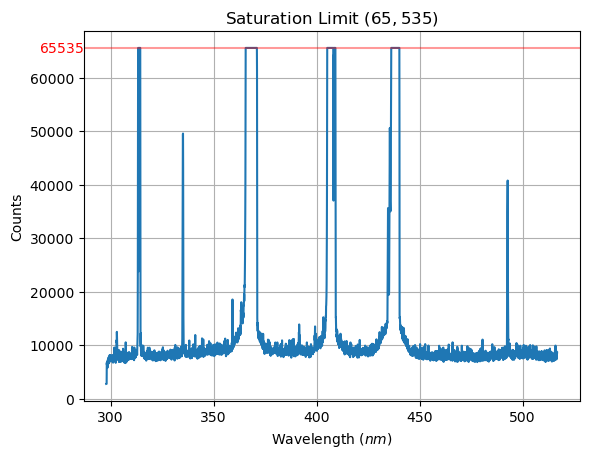
\includegraphics[width=0.7\textwidth]{/home/dj-lawton/Documents/Junior Sophister/JS Labs/Molecular Spectroscopy/Images/Mercury_Saturation_Limit.png}
    \caption{\label{fig:MercurySaturation} The saturation limit of the spectrometer at 65535 counts, as read from the data, visualised.}
\end{figure}
% \vspace{2cm}\\
\indent After capturing the mercury emission spectrum, we found the peaks of the spectrum using the code provided in section \ref{sec:code}, and compared the centres of the Gaussian fits to the literature values. The error takes into account both the spread of the peaks and the accuracy of the fit.\\
\begin{tabular}{p{0.19\textwidth}|p{0.19\textwidth}|p{0.19\textwidth}|p{0.19\textwidth}|p{0.19\textwidth}}
    \hline
    \hline
    Expected\cite{article2} & Measured FLM-T & Expected-Measured FLMT & Measured FLM-S & Expected-Measured FLMS\\
    (nm)& (nm)& (nm)& (nm)& (nm)\\
    \hline
    312.567 & $314.043\pm0.147$ & $1.476\pm0.147$& - & -\\
    334.148 & $335.073\pm0.144$ & $0.925\pm 0.144$ & - & -\\
    365.015 & $365.949\pm0.185$ & $0.935\pm0.185$ & - & -\\
    366.328 & $367.228\pm0.174$ & $0.900\pm0.174$ & $370.264\pm0.617$ & $3.936\pm0.617$\\
    404.656 & $405.456\pm0.166$ & $0.800\pm0.166$ & $409.766\pm0.474$ & $5.110\pm0.474$\\
    407.750 & $408.571\pm0.174$ & $0.821\pm0.174$ & $412.831\pm0.828$ & $5.081\pm0.828$ \\
    435.833 & $436.549\pm0.160$ & $0.716\pm0.160$ & $440.884\pm0.589$ & $5.051\pm0.589$\\
    546.075 & - & - & $550.526\pm0.882$ & $4.451\pm0.882$ \\
    576.961 & - & - & $581.127\pm0.746$ & $4.166\pm0.746$ \\
    579.067 & - & - & $582.873\pm0.965$ & $3.806\pm0.965$ \\
    \hline
    \hline
\end{tabular}
\vspace{1cm}\\
If we assume that the offset is constant, we can take the average of the differences, and add this to any measured spectrum to get the corrected spectrum. These offsets are $(0.939\pm0.0623)nm$ and $(4.514\pm0.282) nm$ for the Flame-T and Flame-S spectrometers, where the error is propogated through the averaging by adding in quadrature, and dividing by sample size.\\
\indent The optical resolution we found using the same fits, since it is related to the standard deviation of the Gaussian fits by
\begin{equation}
    \text{FWHM} = 2\sqrt{2\ln(2)}\sigma
\end{equation}
This then allows to find a value for each peak.\\
% \vspace{0.2cm}\\
\begin{center}
\begin{tabular}{c|c|c|c|c}
    \hline
    \hline
    Expected & \multicolumn{2}{c}{FWHM (nm) - Optical Resolution} & \multicolumn{2}{c}{Resolving Power}\\
    ~ & FLAME-T & FLAME-S & FLAME-T & FLAME-S \\
    \hline
    
    312.155  &  $0.335\pm0.016$ & -        & $931.806\pm44.504$        & -        \\
    334.148  &  $0.328\pm0.017$ & -        & $1018.744\pm52.801$        & -        \\
    365.015  &  $0.391\pm0.018$ & -        & $933.542\pm42.98$        & -        \\
    366.328  &  $0.391\pm0.012$ & $1.432\pm0.122$ & $936.900\pm28.75$ & $ 255.815\pm21.794$\\
    404.656  &  $0.387\pm0.012$ & $1.116\pm0.027$ & $1045.622\pm32.422$ & $362.595\pm8.772$ \\
    407.750  &  $0.421\pm0.015$ & $1.592\pm0.134$ & $968.527\pm34.5$ & $256.124\pm21.56$ \\
    435.833  &  $0.372\pm0.015$ & $1.384\pm0.036$ & $1171.594\pm 47.242$ & $314.908\pm8.19$ \\
    546.075  &  -        & $2.013\pm0.235$ & -        & $271.274\pm31.669$ \\
    576.961  &  -        & $1.741\pm0.249$ & -        & $331.396\pm47.397$ \\
    579.067  &  -        & $2.258\pm0.317$& -        & $256.451\pm36.003$ \\
    
\end{tabular}
\end{center}
This resolution data gives us two plot, against which we fit linear functions.
\begin{figure}[H]
    \centering
    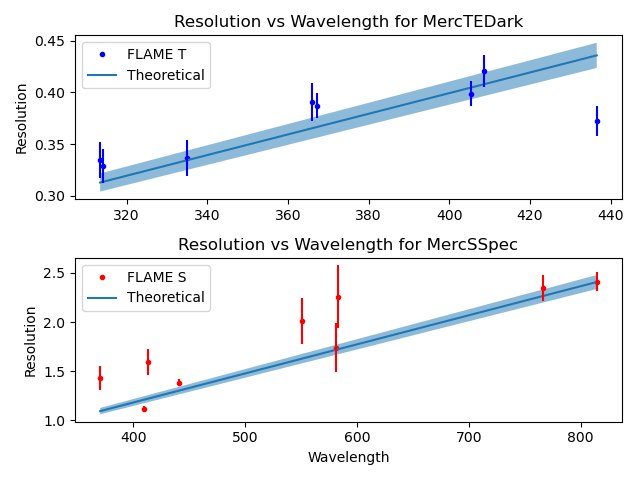
\includegraphics[width=0.7\textwidth]{/home/dj-lawton/Documents/Junior Sophister/JS Labs/Molecular Spectroscopy/Images/ResolutionvsWavelength.png}
    \caption{\label{fig:Resolution} The optical resolution of the Flame-T and Flame-S spectrometers, with a linear fit.}
\end{figure}
This fit gives us a value of $(9.9811\pm0.1395)10^{-4}$ for the slope of the FLAME-T spectrometer fit, and $2.9554\pm0.0436$ for the FLAME-T spectrometer, which are $\frac{1}{R_T}$, $\frac{1}{R_S}$, where $R_T = 1001.894\pm14.007, R_S = 338.359\pm4.993$. This are both well within reasonable proximity of our estimated values above.\\
\subsection{Emission Spectrum of $N_2$}
\section{Discussion}
\newpage
\section{Appendix}

\subsection{Keywords, Mathematical Preliminaries}
\subsubsection{Keywords}
\begin{enumerate}
    \item \textbf{Vibronic Transition:} A transition between vibrational and electronic energy levels.
    
    \item \textbf{Franck-Condon Principle:} The principle that states that an electronic transition is most likely to occur without changes in the positions of the nuclei in the molecular entity and its environment (vibrational, external motion)\cite{MolecularSpectroscopy}.
    
    \item \textbf{Morse Potential:} A potential used to describe the energy levels of a molecule, which accounts for the finite energy $D_e$ which is the depth of the well.
    
    \item \textbf{Molecular Orbital:} An orbital formed from the combination of atomic orbitals of the atoms involved in the molecule.
    
    \item \textbf{Optical Resolution:} Defined as the ability of an optical instrument to distinguish between two objects that are close together. In spectroscopy, we take it to be the full width at half maximum of the peaks.
    
    \item \textbf{Resolving Power:} Defined as the ability of an optical instrument to distinguish between two wavelengths that are close together. In spectroscopy, we take it to be the ratio of the wavelength of the peak to the smallest resolvable difference in wavelengths.
    
    \item \textbf{Wavenumber:} The reciprocal of the wavelength of a wave, expressed in $m^{-1}$.
    
    \item \label{kew:int_time}\textbf{Integration Time:} The time taken to measure the sample.
    
    \item \label{kew:s_t_a}\textbf{Scans to Average:} The number of scans taken to average the sample.
    
    \item \label{kew:binwidth}\textbf{Bin Width:} The width of the bins used to measure the sample.
    
    \item \label{kew: DarkCurrent}\textbf{Dark Current:} The current that flows through the spectrometer when no light is incident on the detector.
    
    \item \textbf{Dissociation Energy:} The energy required to break a bond in a molecule.
    
    \item \textbf{Anharmonicity Constant:} A constant that describes the deviation of a potential from the harmonic oscillator model.
    
    \item \label{kew: ADC}\textbf{ADC:} Analogue to Digital converter, which converts continuous-time, continuous amplitude, voltage input to discrete-time, discrete-amplitude digital output \cite{enwiki:1248045950}.
    
\end{enumerate}
\subsubsection{Mathematical Preliminaries}
\begin{enumerate}
    \item \textbf{Gaussian Distribution:} A continuous probability distribution described by the formula:
    \begin{equation}
        g(x) = Ae^{-\frac{(x-x_0)^2}{2\sigma^2}}
    \end{equation}
    where $A$ is the amplitude, $x_0$ is the mean, and $\sigma$ is the standard deviation.
\end{enumerate}
\subsection{Code}\label{sec:code}
All code used in this experiment can be found at \url{https://github.com/DavidLawton04/MuchStuff/tree/a66c3f8d47b7b2ac18273ab8eca6349f52667f22/Junior%20Sophister/JS%20Labs/Molecular%20Spectroscopy}




\bibliographystyle{plain}
\bibliography{references}

\end{document}